\chapter{Implementation}
\label{chapter:Implementation}
This chapter summarizes the implementation of crucial parts of recovery system implemented for this thesis.
§\ref{section:RecoveringFragments} covers the implementation of \gls{Fragment} recovery.
§\ref{section:RecoveryOfParthoodLinks} covers the implementation of \gls{Parthood} link recovery.
§\ref{section:RecoveryOfCorrespondenceAndConformanceLinks} covers the implementation of \gls{Correspondence} and \gls{Conformance} link recovery

\section{Recovering Fragments}
\label{section:RecoveringFragments}
This section summarizes the implementation of \gls{Fragment} recovery.
\Glspl{Fragment} are syntactically well-formed pieces of code.
For instance, consider the following \gls{Java} class:
\begin{lstlisting}[language=Java,numbers=none]
public class Company {
	...
	private String name;
	...
	public String getName() {
		return name;
	}
	...
}
\end{lstlisting}
It consists of the following fragments among others:
\begin{itemize}
\item
a field declaration fragment for \texttt{name}:
\begin{lstlisting}[language=Java,numbers=none]
private String name;
\end{lstlisting}
\item
a method declaration fragment for an accessor-method of \texttt{name}:
\begin{lstlisting}[language=Java,numbers=none]
public String getName() {
	return name;
}
\end{lstlisting}
\item
the return statement of the accessor-method:
\begin{lstlisting}[language=Java,numbers=none]
return name;
\end{lstlisting}
\item
the class declaration itself can also be considered a fragment.
\end{itemize}

The task of recovering \glspl{Fragment} is to add entities for each of such code pieces into a megamodel.
Figure \ref{figure:IdealizedRecoveryOfJavaFragments} exemplifies the recovery of \gls{Java} \glspl{Fragment} in an idealized form.
\begin{figure}[h!]
\begin{center}
\begin{minipage}{0.5\textwidth}
\begin{lstlisting}[language=Java,numbers=none]
public class Company {
	...
	private String name;
	...
	public String getName() {
		return name;
	}
	...
}
\end{lstlisting}
\end{minipage}
\\\vspace*{5mm}
{
\LARGE
\bfseries
$\downarrow$
}
\\\vspace*{5mm}
\resizebox{\textwidth}{!}{
\Tree [.Class \texttt{public} \texttt{class}
	[.ID \texttt{Company} ]
	\texttt{$\lbrace$}
	[.Members 
		[.Member \texttt{...} ]
		[.Member \texttt{public} \texttt{String} [.ID \texttt{name} ] \texttt{;} ]
		[.Member \texttt{...} ]
		[.Member \texttt{public} \texttt{String} [.ID \texttt{getName} ] \texttt{(} \texttt{)}
		\texttt{$\lbrace$}
		[.Statements
			[.Statement \texttt{return} \texttt{name} \texttt{;} ]
		]
		\texttt{$\rbrace$}
		]
		[.Member \texttt{...} ]
	]
	\texttt{$\rbrace$}
]
}
\\\vspace*{5mm}
{
\LARGE
\bfseries
$\downarrow$
}
\\\vspace*{5mm}
\resizebox{\textwidth}{!}{
\Tree [.Class
[.\texttt{public class Company \{ private String name; public String getName() \{ return name; \} \}}
	[.Fields 
		[.Field \texttt{...} ] 
		[.Field \texttt{private String name;} ] 
		[.Field \texttt{...} ] 
	]
	[.Methods 
		[.Method \texttt{...} ]
		[.Method \texttt{public String getName() \{ return name; \}} ]
		[.Method \texttt{...} ]
	]
]]
}
\\\vspace*{5mm}
{
\LARGE
\bfseries
$\downarrow$
}
\\\vspace*{5mm}
\begin{minipage}{0.5\textwidth}
\begin{lstlisting}[numbers=none]
Company : Fragment
Company elementOf JavaClassFragments
...
Company.name : Fragment
Company.name elementOf JavaFieldFragments
...
Company.getName : Fragment
Company.getName elementOf JavaMethodFragments
\end{lstlisting}
\end{minipage}
\end{center}
{
\scriptsize
This picture shows an idealized recovery of \gls{Java} \glspl{Fragment}:
\begin{center}
code \gls{Artifact}
$\rightarrow$
\gls{ParseTree}
$\rightarrow$
\gls{Fragment} \gls{AST}
$\rightarrow$
\gls{Megamodel}
\end{center} 
Both \gls{ParseTree} and \gls{AST} are depicted in a simplified, schematic form.
}
\caption{Idealized Recovery of Java Fragments}
\label{figure:IdealizedRecoveryOfJavaFragments}
\end{figure}
\begin{enumerate}
\item
a \gls{ParseTree} is generated from an artifact; this is done via \gls{ANTLR} as described in §\ref{subsubsection:SyntaxAnalysisAPI} and does not require further explanation, since it is only an application of the most common \gls{ANTLR} use case
\item
then the \gls{ParseTree} is transformed into an concrete \gls{Fragment} \gls{AST} model; this is also done relying on \gls{ANTLR} tree traversal utilities and described in detail in §\ref{subsection:ConcreteFragmentASTModels}
\item
eventually, nodes of the generated \gls{Fragment} \gls{AST} are added to a \gls{Megamodel} as entities; the details are described in §\ref{subsection:MegamodelingFragments}.
\end{enumerate}

Note, fragment Recovery for \gls{XML} and \gls{SQL/DDL} is implemented in a similar fashion.
If there is a noteworthy difference for other languages it will be explored, otherwise we keep using \gls{Java} as example domain for the following sections of §\ref{section:RecoveringFragments}.

\subsection{Concrete Fragment AST Models}
\label{subsection:ConcreteFragmentASTModels}
As mentioned in §\ref{subsubsection:AbstractFragmentModel}, Concrete \Gls{Fragment} \gls{AST} Models are derivations of the Abstract Fragment Model of the Recovery System \gls{API}.
Figure \ref{figure:JavaFragmentASTModel} shows an \gls{UML} class diagram of the implemented \Gls{Fragment} \gls{AST} for \gls{Java}.
\begin{figure}[h!]
\begin{center}
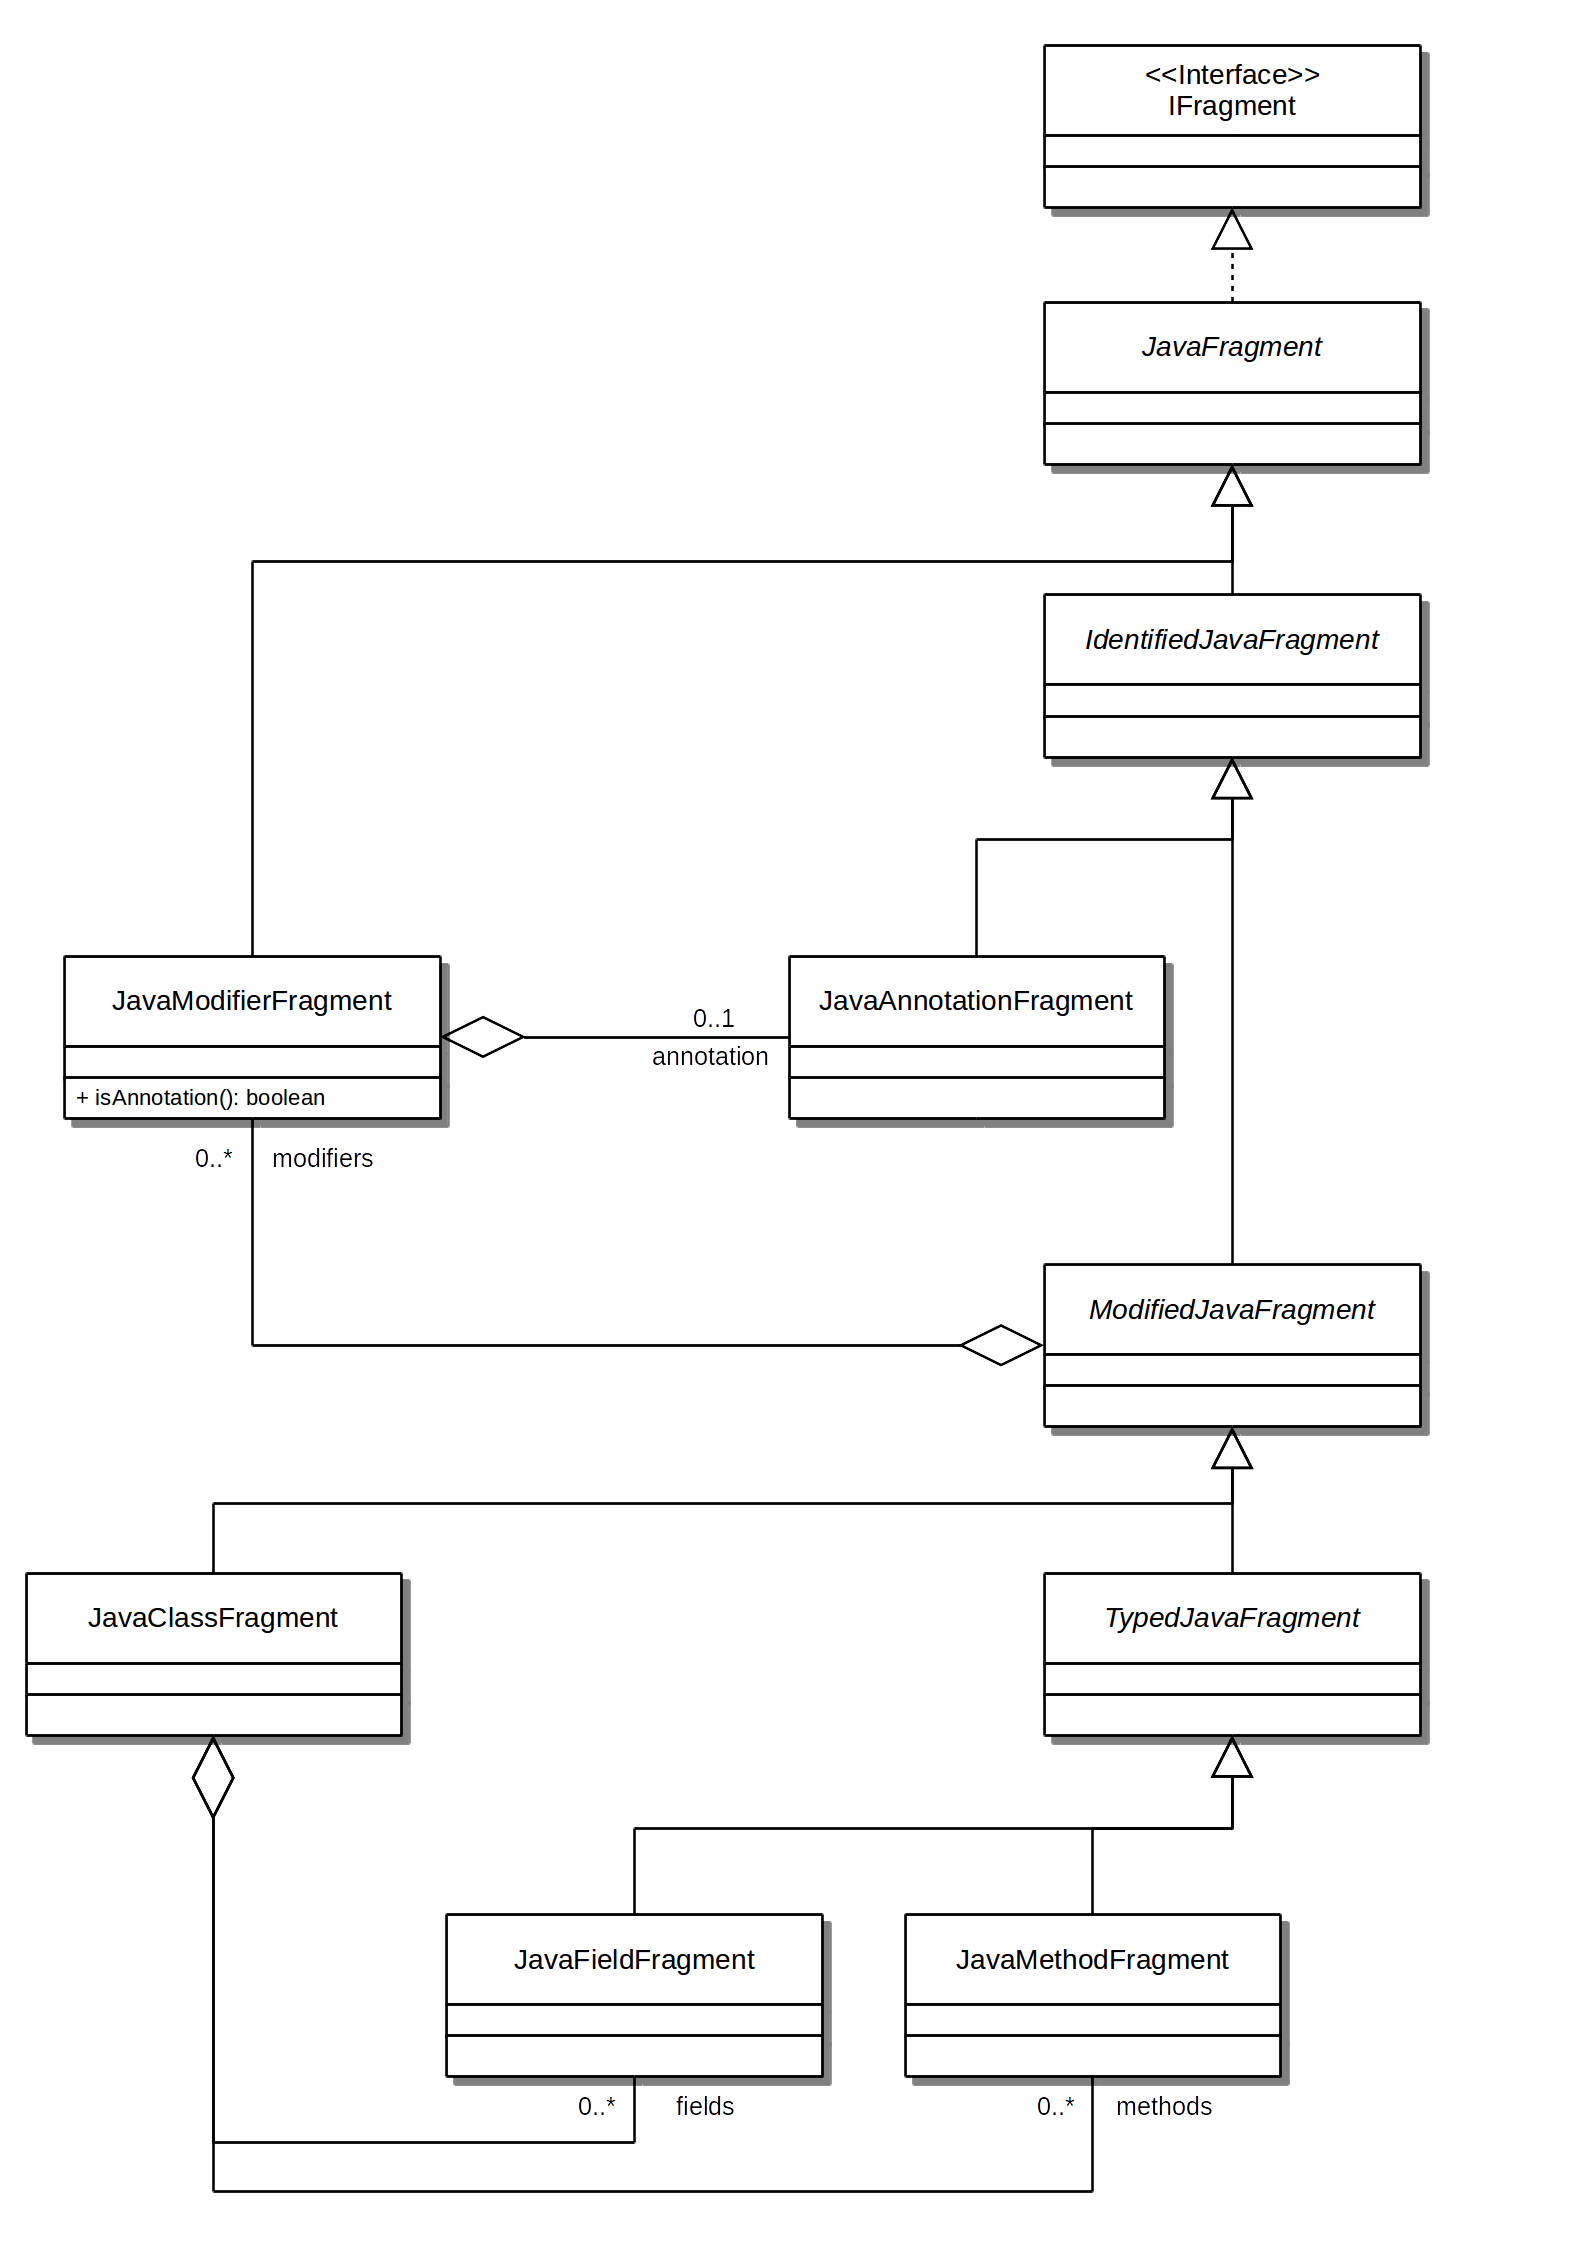
\includegraphics[width=.7\textwidth]{images/JavaFragmentModel.png}
\end{center}
\caption{Java Fragment AST Model}
\label{figure:JavaFragmentASTModel}
\end{figure}
All \gls{Fragment} classes derive from \text{IFragment} through the base class \texttt{JavaFragment}.
From here, several specializations are introduced:
\begin{itemize}
\item
\texttt{IdentfiedJavaFragment} for constructs with identifiers
\item
\texttt{ModifiedJavaFragment} for constructs with modifiers like \texttt{private}, \texttt{public}, \texttt{final}, \texttt{abstract}, \texttt{static}, etc. or annotation meta-data
\item
\texttt{TypedJavaFragment} for constructs with distinct (return-) type like fields, methods or variables
\end{itemize}
Note, the \gls{Fragment} model for \gls{Java} only focuses on structural syntactical features of the language.
Everything below method signature level is omitted, because \glspl{Fragment} of this level are not important for the scope of this thesis.
On the other hand, annotations are captured, since they provide significant information for further recovery analysis.
\gls{Hibernate} and \gls{JAXB} rely on annotations for \gls{O/R/X-Mapping}.

The \gls{AST} is constructed using \gls{ANTLR} \texttt{ParseTreeListener} approach as described in §\ref{subsubsection:SyntaxAnalysisAPI}.
Figure \ref{figure:JavaFragmentASTConstruction} shows an excerpt from the listener implementation used to construct the the \gls{AST} for \gls{Java} \glspl{Fragment}.
\begin{figure}[h!]
\begin{lstlisting}[language=Java]
...
@Override
public void exitMethodDeclaration(Java8Parser.MethodDeclarationContext ctx) {
    javaMethodFragments.push(java8FragmentFactory.newJavaMethodFragment(ctx, javaMethodModifierFragments));
}

@Override
public void exitNormalClassDeclaration(Java8Parser.NormalClassDeclarationContext ctx) {
    javaClassFragments.push(java8FragmentFactory.newJavaClassFragment(ctx, javaClassModifierFragments, javaFieldFragments, javaMethodFragments, declaredPackage));
}
...
\end{lstlisting}
{
\scriptsize
This snippet shows an excerpt of the listener used to construct \gls{Java} \gls{Fragment} \glspl{AST}.
}
\caption{Construction of Java Fragment ASTs}
\label{figure:JavaFragmentASTConstruction}
\end{figure}
Here, fragment instances are created when the listener leaves a certain node of the \gls{ParseTree}.
Creation is delegated to a factory.
The listener pushes fragments onto stacks, making the overall implementation work like a pushdown automaton or stack machine.



\subsection{Megamodeling Fragments}
\label{subsection:MegamodelingFragments}
asdf
\begin{figure}[h!]
\begin{lstlisting}
...
Language < Set
...
fragmentLanguageOf < Language * Language
...
Java : Language

JavaFragments : Language
JavaFragments fragmentLanguageOf Java

JavaClassFragments : Language
JavaClassFragments subsetOf JavaFragments

JavaFieldFragments : Language
JavaFieldFragments subsetOf JavaFragments

JavaMethodFragments : Language
JavaMethodFragments subsetOf JavaFragments
...
\end{lstlisting}
{
\scriptsize
}
\caption{A \Gls{Megamodel} for \Gls{Java} \Glspl{Fragment}}
\label{figure:JavaFragmentMegamodel}
\end{figure}


\section{Recovering Parthood Links}
\label{section:RecoveryOfParthoodLinks}
This section summarizes the implementation of \gls{Parthood} link recovery.





\section{Recovering Correspondence \& Conformance Links}
\label{section:RecoveryOfCorrespondenceAndConformanceLinks}
This section the implementation of \gls{Correspondence} and \gls{Conformance} link recovery